\chapter{Background}\label{chap:background}
The title of this thesis is \textit{\thesisTitle}.
It brings together the domains of Process Science, Predictive Modeling and Deep Learning.
This chapter gives insights into the parts of these topics that will be used and needed throughout the thesis.
This work can be attributed to the domain of Predictive Process Monitoring, which will also be introduced.

\section{Process Science And Process Monitoring}
Process Science, as loosely defined by van der Aalst \cite{Aalst2016}, refers to the \textit{broader discipline that combines knowledge from information technology and knowledge from management sciences to improve and run operational processes}. This means that approaches in this domain tend to be driven by models, such as Six Sigma or Kaizen\todo{source?}.

Central to process science is Business Process Management (BPM) which is squarely aimed at improving operational business performance through the optimization of business processes via their models.
Modeled e.g. with the Business Process Modeling Notation (BPMN) \cite{bpmn2.0}, these models are typically very rigid and permit little variation of the workflow. The central element of these notations are the individual steps of which a process is comprised, referred to as \textit{activities}, as also shown in \ref{fig:activity-introduction}.

\begin{figure}
    \centering
    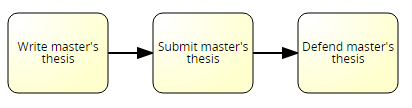
\includegraphics[width=.75\textwidth]{gfx/activity-introduction.png}
    \caption{The yellow boxes and their description are used in BPMN to describe an activity. The arrows denote the control flow in between.}
    \label{fig:activity-introduction}
\end{figure}

With the help of workflow management systems (WFMS), it became possible to embed and enforce these structured processes in an organization, making them traceable via the logs that these systems generated. 

Especially in the insurance and health-care sector, each case tended to be very different from the next \cite{hewelt2016}. This led to the notion that the course of a case strongly depends on the information contained inside it.

\subsection{Case Management}
In settings in which it is common to employ BPM, such as assembly line productions, there is little heterogeneity. As the latter increases, BPMN and other business process modeling notations result in complex and hardly understandable models and thus fail their purpose. As previously mentioned, this tends to occur in domains where the case trajectory is highly dependant on information contained inside it.

The fact that this type of process is data-driven led to the creation of the \textit{case folder} - a directory central to a case, describing its current state. In Case Management (CM), the process acts on the data contained inside this folder, making it have a direct impact on the course of a case. In contrast to BPM, the formalization of Case Management and the subsequent creation of modeling languages has only just begun. Notable developments include the Case Management Modeling Notation \cite{web:cmmn} as well as the Chimera approach \cite{hewelt2016}.
\todo[inline]{graphical illustration of case}

\subsection{Process Mining}
The logs generated through the users actions give rise to the discipline of Process Mining, which covers the three steps of model discovery, conformance checking and model enhancement \cite{Aalst2016}. They are enabled through the use of techniques from the area of Data Science, making it possible to understand Process Mining as the link between Data Science and Process Science as in \autoref{fig:process-data-science}. An excerpt from a log is depicted in figure \ref{fig:process-log}.

A major problem in this domain pose \textit{spaghetti} and \textit{lasagna} models. Such overly complex and unreadable models are mined from process logs that contain highly variable execution traces. Such logs often come from CM executions.

\begin{figure}
    \centering
    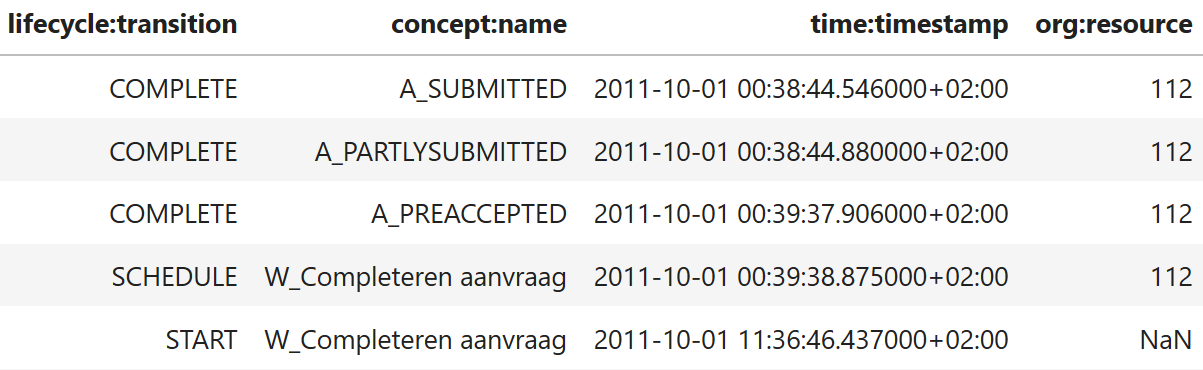
\includegraphics[width=\textwidth]{gfx/process-log}
    \caption{The first entries of an exemplary event log from a case from the BPIC 2011 dataset\cite{BPIC2011}. Each event is associated with data and the column \texttt{concept:name} corresponds to the activity title.}
    \label{fig:process-log}
\end{figure}

\subsection{Predictive Process Monitoring}
In parallel to this development, WFMS already permitted the unstructured execution of processes, empowering the user to make the best choice about which activity to do next. The knowledge to do so made him or her the \textit{knowledge worker}.
As Process Mining is concerned with data-driven process discovery and optimization only on offline data, a possibility to act on case developments in real-time is desirable. Commonly referred to as \textit{Predictive Process Monitoring} \cite{francescomarino2015, schoenig2018}, the application of predictive analytics on running and thus incomplete case logs fulfills this need. Connecting two subdomains of Process Science and Data Science, this is what sets it apart from Process Mining \autoref{fig:process-data-science}.

\begin{figure}
    \centering
    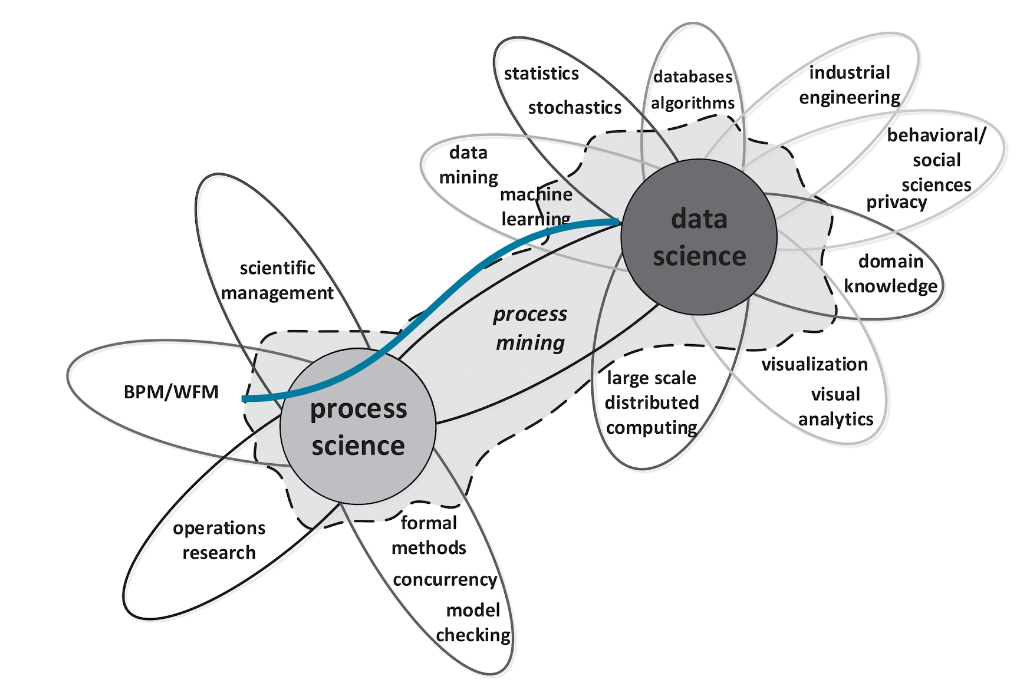
\includegraphics[width=\textwidth]{gfx/process-data-science.png}
    \caption{Process Mining can be understood as the bridge between Process Science and Data Science \cite[p.18]{Aalst2016}. The blue line symbolizes the subdomains that Predictive Process Monitoring brings together.}
    \label{fig:process-data-science}
\end{figure}

Instead of revolving around models, this discipline is concerned with predicting certain characteristics of the running case that lie in its future. This allows answering questions such as:

\begin{itemize}
    \item Will I still meet my service level agreement?
    \item Will we be able to deliver the package in within our 3-hour target?
    \item How long is this case still going to take?
    \item What is going to be the next step?
\end{itemize}

The answers to these questions can give case workers the opportunity to intervene if a case takes an unwanted course or might fail to meet KPI requirements. Furthermore, this approach only requires sufficient amounts of historical case executions, but no model. While it can certainly be a useful addition, it is not needed. 

%\begin{figure}
%	\centering
%	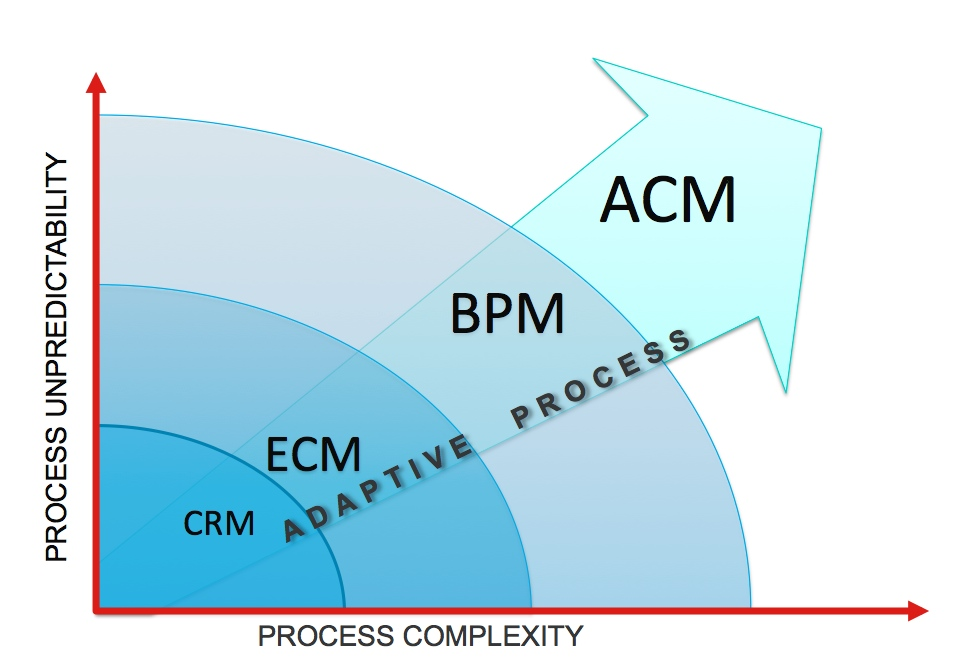
\includegraphics[width=\textwidth]{gfx/acm-reasoning}
%	\caption{https://acmisis.wordpress.com/what-is-adaptive-case-management-acm/}
%	\label{fig:why-acm}
%\end{figure}

\section{Predictive Modeling}
Predictive modeling is a process that uses data mining and learned statistical properties of the data, henceforth referred to as predictive models, to forecast outcomes. It is important to note that predictive models are unrelated to process models. This section shall introduce a common process for predictive model generation and frame a problem that is fundamental to the thesis: that of next-element predictions in a sequence.

\subsection{Predictive model development}
A predictive model takes in a number of \textit{features}, which are variables that are likely to influence the prediction of the \textit{target variable}. Features are sometimes also referred to as predictor variables.
These features are often \textit{engineered}, i.e. aggregated, or differently encoded to assist the model during learning.

The model itself can be chosen from a wide array of possibilities, such as linear regressions, decision trees, random forests, scalable vector machines (SVM) or neural networks (NN).

Once features and model are chosen, the model is \textit{trained} on the dataset. During this training phase, the model uses accuracy metrics to assess the quality of its predictions, learn the statistical properties of the data and adjust itself internally accordingly. Certain input parameters of the model are adjusted during this phase as well, an activity referred to as \textit{hyper-parameter tuning}. Training the model can be a very time-consuming task, unless appropriate hardware is used. Such hardware might be specially designed for model learning (i.e. Google's Tensor Processing Units) or a simple Graphics Processing Unit (GPU).

As predictors, model choice and hyper-parameters have a strong impact on model quality, these steps are frequently iterated upon, as Fayyad et al. discovered \cite{fayyad1996data}. The process for model development they discovered 20 years ago is illustrated in \autoref{fig:kdd_process} and as current as ever.

\begin{figure}
	\centering
	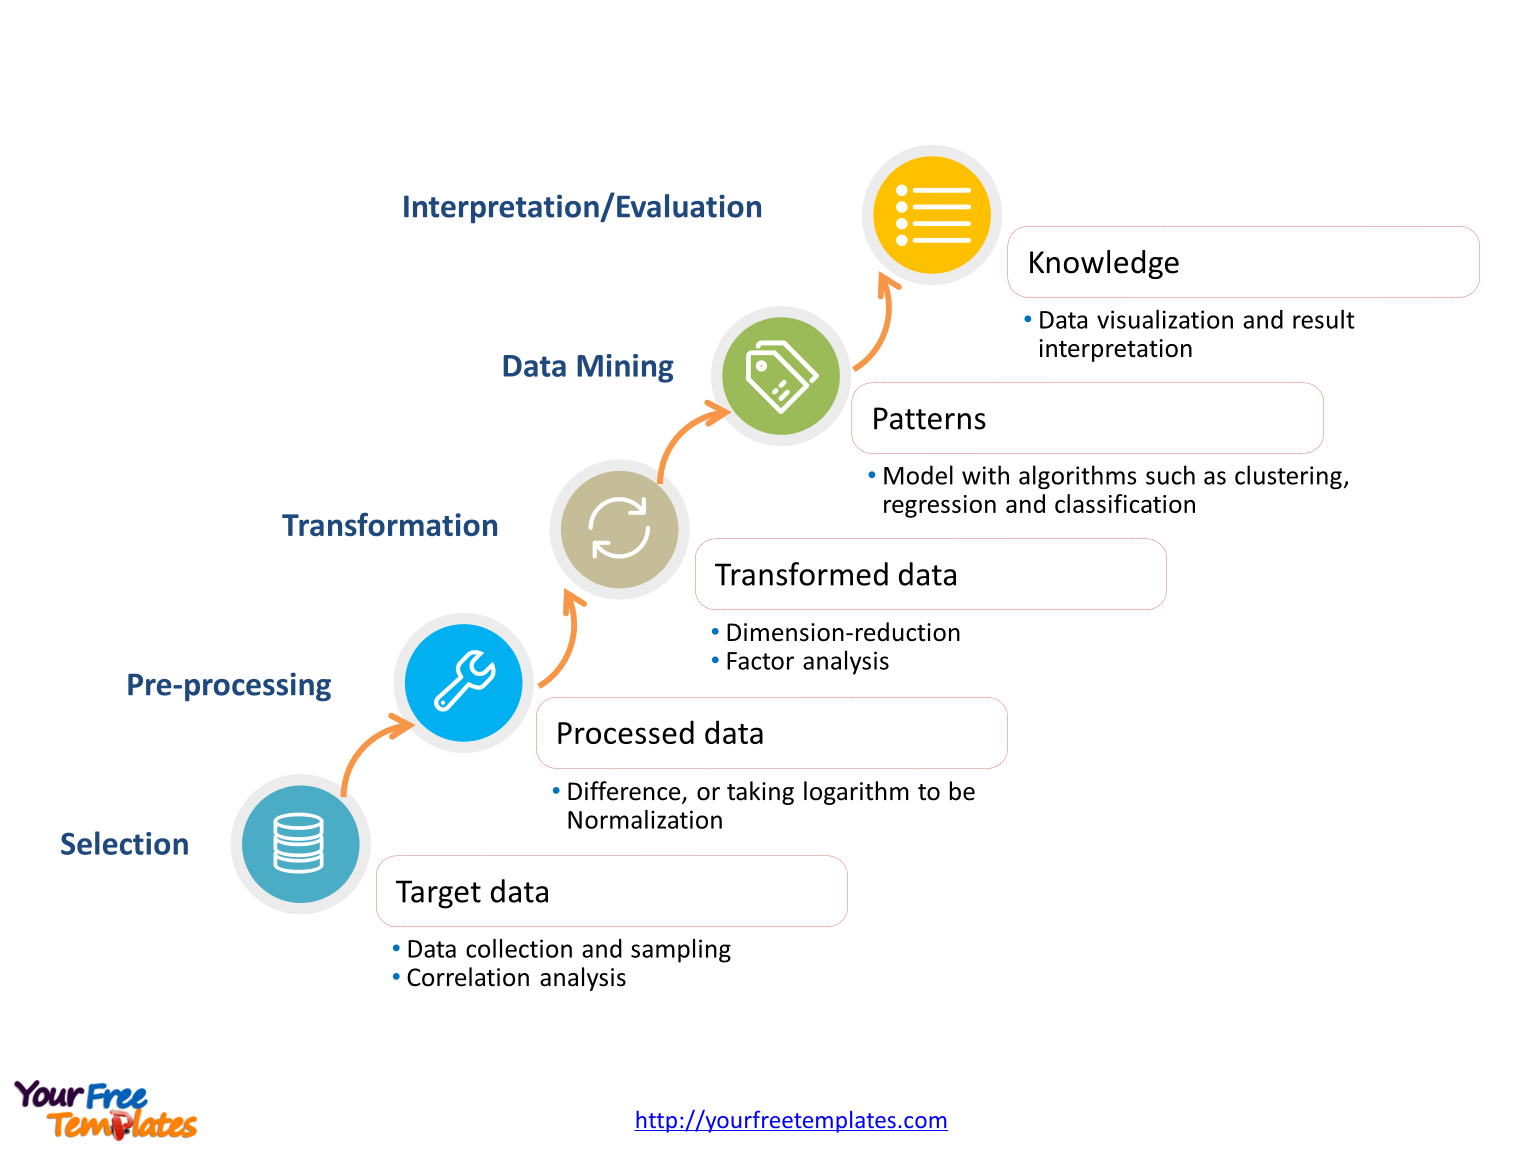
\includegraphics[width=\textwidth]{gfx/kdd_process}
	\caption{The process for \textit{Knowledge Discovery in Databases} as per Fayyad et al. \cite{fayyad1996data}.}
	\label{fig:kdd_process}
\end{figure}

\subsection{Sequence prediction}
In this section, a formal definition of sequences is presented, and then set in relation with the problem at hand\footnote{Definition adapted from \cite{pei2001prefixspan}}.  Let $I = \{i_1,i_2,...i_n\}$ be the set of all items. An \textit{itemset} is a subset of $I$. A \textit{sequence} is an ordered list of itemsets, such that in its notation $seq = \langle s_1s_2...s_l \rangle$, the following rule holds: $\forall\ 1 \leq j \leq l: s_j \subseteq I$. Then, $S$ defines the infinite set of all possible sequences. It is infinite because sequences can be arbitrarily long, with each itemset containing an arbitrary number of items.

Assuming that a a sequence can be finished, consider the database of completed sequences $DS$. Under the assumption of the Markovian hypothesis that "[...] the probability of each event depends only on the state attained in the previous event"\footnote{Gagniuc, Paul A. (2017). Markov Chains: From Theory to Implementation and Experimentation. USA, NJ: John Wiley \& Sons. pp. 1–235. ISBN 978-1-119-38755-8.}, a predictive model is be trained on this database to predict the next sequence $nseq$ or itemset $s_k$ of an incomplete sequence $seq_{inc}$:

\begin{equation}
\begin{split}
    predict(seq_{inc}) &= \widehat{nseq}\\ predict(seq_{inc}) &= \hat{s_k}\ |\ 1 \leq k \leq l
\end{split}
\label{eq:prediction-from-sequence}
\end{equation}

Sequence predictions are a common problem in the domains of machine translation and text generation. For example, the translation of the sentence \textit{"I am writing my master's thesis"} into the german sentence \textit{"Ich schreibe meine Masterarbeit"} can easily be mapped onto the notation previous described. With $I$ being the alphabet and punctuation marks and each itemset representing a single word, the input and target sequences could be noted as:

\begin{equation*}
\begin{split}
seq_{in} &= \langle<I>, < >, <am>, ... <thesis>\rangle\\
seq_{out} &= \langle<Ich> ... <Masterarbeit>\rangle
\end{split}
\end{equation*}

Referring to the \autoref{eq:prediction-from-sequence}, $seq_{in}$ can be understood as $seq_{inc}$ and $seq_{out}$ as $\widehat{nseq}$. This was an example of a classic \textit{sequence-to-sequence} prediction.

Next to this kind of prediction, there are also \textit{sequence-to-word} predictions, which can be used to generate text and even write simple novels.

However, the next itemset of a sequence need not be a word - it can also be an activity of a business process still running. The formal transfer of sequence prediction to business processes shall be presented in \autoref{sec:contribution}, as it is an important part of the contribution.

Predictive models such as random forests take inputs of fixed size. Unfortunately, sequences can be of arbitrary length, and thus the \textit{curse of dimensionality} also appears in context with this problem. To bring variable length inputs into a format that can be processed by predictive models (such as in \autoref{fig:process-log}), several data input formats have been invented. As their names suggest, these come from the domain of Natural Language Processing (NLP), but can easily be transferred to the problem at hand. These shall be briefly introduced in the following:

\subsubsection{Sliding Window}
\subsubsection{N-gram}
\subsubsection{Bag-Of-Words}
\subsubsection{Learned features, word2vec}
Strictly piecewise\\
subsequences, embedding
PrefixSpan

\section{Neural networks}
give insights into deep learning and neural networks 

follow explanation of colah.github.io

\subsection{RNN}
\subsection{LSTM memory}